\begin{figure}[h!]
\centering
\sidecaption{.63\textwidth}{.35\textwidth}{
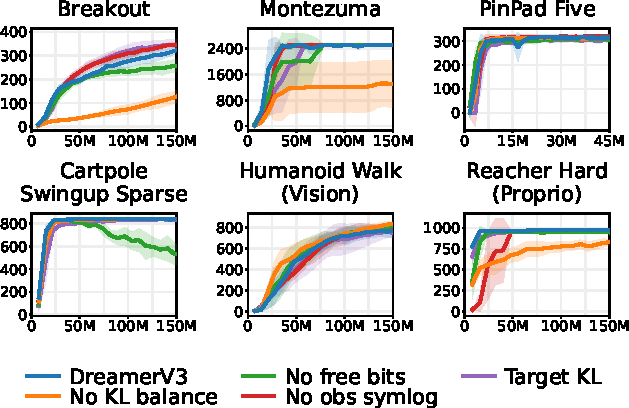
\includegraphics[width=\linewidth]{ablations/ablation_model}}{
\caption{World Model ablations. KL balancing \citep{hafner2020dreamerv2} subsantially accelerates learning. Free bits \citep{kingma2016freebits,hafner2019dreamer} avoids overfitting in simple environments. Symlog encoding and predictions for proprioceptive observations speeds up learning. Adjusting the KL scale over the course of training within a reasonable range to target a fixed KL value is a performant but more complicated alternative to free bits.}
\label{fig:ablation_model}}
\end{figure}
\vspace*{.5ex}

\begin{figure}[h!]
\centering
\sidecaption{.63\textwidth}{.35\textwidth}{
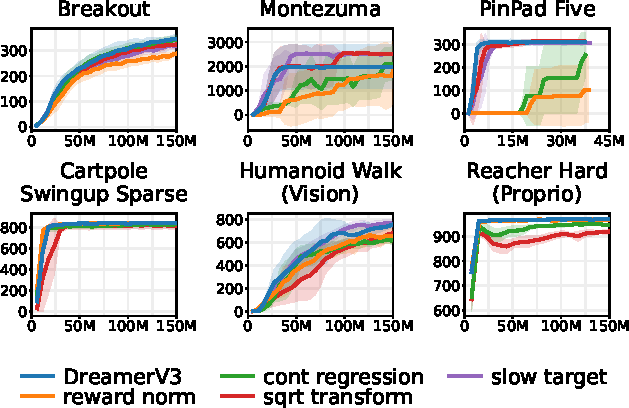
\includegraphics[width=\linewidth]{ablations/ablation_critic}}{
\caption{Critic ablations. The symlog predictions for rewards and values in DreamerV3 outperform non-stationary reward normalization. Discrete regression also contributes significantly \citep{schrittwieser2019muzero}. Symlog transformation slightly outperforms the more complex asymmetric square root transformation of R2D2 \citep{kapturowski2018r2d2}. Using the slow critic for computing targets offers no benefit over using the fast critic and regularizing it towards its own EMA.}
\label{fig:ablation_critic}}
\end{figure}
\vspace*{.5ex}

\begin{figure}[h!]
\centering
\sidecaption{.63\textwidth}{.35\textwidth}{
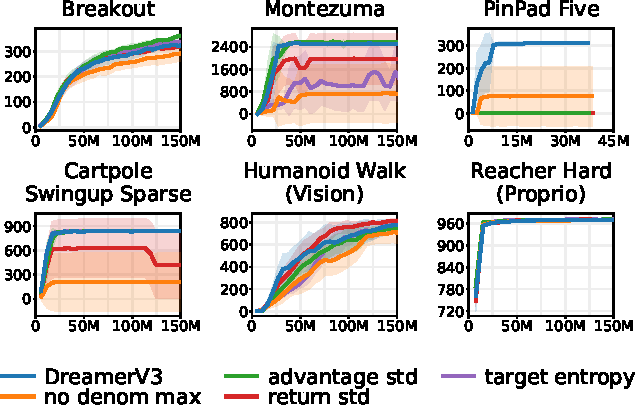
\includegraphics[width=\linewidth]{ablations/ablation_actor}}{
\caption{Actor ablations. The strength of the actor entropy regularizer is important especially under sparse rewards, where the right amount of stochasticity is needed for exploration. The denominator maximum that prevents small returns (often noise) from being amplified is critical. The percentile return normalization of DreamerV3 outperforms normalization based on return stddev or advantage stddev on the sparse reward tasks \citep{hafner2022director}.}
\label{fig:ablation_actor}}
\end{figure}
